\documentclass{standalone}
\usepackage{chez}

\begin{document}
\chapter{October 16, 2020}

\begin{example}
  The \(\ZZ\)-module \(\ZZ/2\ZZ \otimes_\ZZ \ZZ/3\ZZ\) has generators
  \[
    0 \otimes 0, \qquad
    1 \otimes 0, \qquad
    0 \otimes 1, \qquad
    1 \otimes 1, \qquad
    0 \otimes 2, \qquad
    1 \otimes 2.
  \]
  We know that
  \[
    0 \otimes 0 =
    0 \otimes 1 =
    0 \otimes 2 =
    1 \otimes 0 = 0,
  \]
  and
  \[
    1 \otimes 1 + 1 \otimes 1 = 1 \otimes (1 + 1) = 1 \otimes 2.
  \]
  Therefore,
  \(\ZZ/2\ZZ \otimes_\ZZ \ZZ/3\ZZ\) is generated by \(1 \otimes 1\).
  However, we know
  \begin{align*}
    1 \otimes 1 + 1 \otimes 1 + 1 \otimes 1 &= 1 \otimes 3 = 0 \\
                  1 \otimes 1 + 1 \otimes 1 &= 1 \otimes 2 = 0,
  \end{align*}
  so \(1 \otimes 1 = 0\).
  Therefore, \(\ZZ/2\ZZ \otimes_\ZZ \ZZ/3\ZZ \iso 0\).
\end{example}

\begin{proposition}
  If \(A\) is an abelian group, then
  \[
    \ZZ/2\ZZ \otimes_\ZZ A \iso A/2A.
  \]
\end{proposition}
\begin{proof}
  The \(\ZZ\)-module \(\ZZ/2\ZZ \otimes_\ZZ A\) is generated by the symbols
  \(1 \otimes a\) for all \(a \in A\) with the relation
  \[
    2(1 \otimes a) = 2 \otimes a = 0 \otimes a = 0. \pog
  \]
\end{proof}

\begin{corollary}
  In general, we have \(\ZZ/n\ZZ \otimes_\ZZ A \iso A/nA\).
\end{corollary}

How about \(\ZZ \otimes_\ZZ A\)?
We know that if \(B\) is an abelian group,
\[
  \Hom(A \otimes_\ZZ \ZZ, B) \iso \Hom(A, \ul\Hom(\ZZ, B)).
\]
Note that \(\ul\Hom_\cAb(\ZZ, B) \iso B\),
because \(\ZZ\) has one generator.
Therefore,
\[
  \Hom(A \otimes_\ZZ \ZZ, B) \iso \Hom(A, B),
\]
and this suggests that \(\ZZ \otimes_\ZZ A \iso A\).
Taking \(B = 0\) gives the result, because \(\ul\Hom(X, 0) \iso X\).

\begin{theorem}
  If \(R\) is a commutative ring and \(M \) is an \(R\)-module, then
  \[
    R \otimes_R M \iso M.
  \]
\end{theorem}

\begin{definition}
  Suppose \(R\) is a ring, and \(A, B, C\) are \(R\)-modules.
  A \vocab{bilinear map} \(f \colon A \times B \to C\) is a function of sets
  such that
  \begin{enumerate}[nosep]
    \item \(f(a + a', b) = f(a, b) + f(a', b)\),
    \item \(f(a, b + b') = f(a, b) + f(a, b')\), and
    \item \(f(r a, b) = r f(a, b) = f(a, r b)\).
  \end{enumerate}
\end{definition}
\begin{lemma}
  Bilinear maps \(A \times B \to C\) are in bijection with
  \(R\)-module maps \(A \otimes_R B \to C\).
\end{lemma}

\begin{theorem}
  Suppose \(A, B, C\) are \(R\)-modules. Then
  \begin{align*}
    (A \oplus B) \otimes_R C &\iso
      (A \otimes_R C) \oplus (B \otimes_R C) \\
    (a, b) \otimes c &\leftrightarrow (a \otimes c, b \otimes c).
  \end{align*}
\end{theorem}

This means that \((\oplus_R, \oplus_R)\) make \(\cRmod\) into
a \vocab{categorical ring}, or a \vocab{ring object in categories}.
In particular, \(\otimes_R\) is associative in the sense that
\[
  (A \otimes_R B) \otimes_R C \iso A \otimes_R (B \otimes_R C).
\]

We now know how to compute \(\otimes_\ZZ\) of
finitely generated abelian groups.

\begin{example}
  \begin{align*}
    (\ZZ/2\ZZ \oplus \ZZ/3\ZZ) \otimes_\ZZ (\ZZ/6\ZZ \oplus \ZZ) &\iso
      (\ZZ/2\ZZ \otimes \ZZ/6\ZZ) \otimes
      (\ZZ/2\ZZ \otimes \ZZ/6\ZZ) \otimes
      (\ZZ/3\ZZ \otimes \ZZ) \otimes
      (\ZZ/3\ZZ \otimes \ZZ) \\
    &\iso \ZZ/2\ZZ \oplus \ZZ/3\ZZ \oplus \ZZ/2\ZZ \oplus \ZZ/3\ZZ
  \end{align*}
\end{example}

The most common abelian groups are finitely generated,
so this is enough for us.

We also want to be able to calculate homology in other rings.
The rings \(R\) we use often in algebraic topology are
\(\ZZ\), \(\QQ\), or a finite field.
Since all non-\(\ZZ\) rings are fields,
these \(R\)-modules are just vector spaces,
which are easy to compute the tensor products of.

\begin{example}
  In \(\QQ\)-modules, what is
  \((\QQ \oplus \QQ) \otimes_\QQ (\QQ \oplus \QQ \oplus \QQ)\)?

  This is a \(6\)-dimensional \(\QQ\)-vector spaces, i.e.\
  \(\QQ \oplus \QQ \oplus \QQ \oplus \QQ \oplus \QQ \oplus \QQ\).
\end{example}

\section{Tensor products of chain complexes}
Let's give a topological example to give some intuition
on how tensor products of chain complexes will work.
\begin{example}
  Consider the interval \(I = [0, 1] = D^1\) as a CW complex.
  \begin{center}
    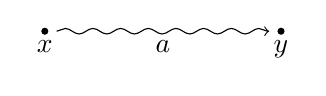
\begin{tikzpicture}[scale=3]
      \draw[decorate, ->, decoration={snake, amplitude=1}]
            (0.05, 0) -- (0.95, 0) node[midway, below]{\(a\)};
      \fill (0, 0) circle[radius=0.015];
      \fill (1, 0) circle[radius=0.015];
      \node[below] () at (0, 0) {\(x\)};
      \node[below] () at (1, 0) {\(y\)};
    \end{tikzpicture}
  \end{center}
  \[
    \Ccell_*(I) \iso \bigg(
    \begin{tikzcd}[row sep=0.1ex]
    	\ZZ\fgen{a} \ar[r] &
        \ZZ\fgen{x, y} \\
    	a \ar[r, mapsto] &
        y - x
    \end{tikzcd}
    \bigg)
  \]
  There is a product cell decomposition for \(I \times I\)
  \begin{center}
  
    \begin{tikzpicture}[scale=2.5]
      \fill[gray!20, path fading=north] (0, 0) rectangle +(1, 1);
      \draw[decorate, ->, decoration={snake, amplitude=1}]
            (0.05, 0) -- (0.95, 0) node[midway, below]{\(a \otimes x\)};
      \draw[decorate, ->, decoration={snake, amplitude=1}]
            (0.05, 1) -- (0.95, 1) node[midway, above]{\(a \otimes y\)};
      \draw[decorate, ->, decoration={snake, amplitude=1}]
            (0, 0.05) -- (0, 0.95) node[midway, left]{\(x \otimes a\)};
      \draw[decorate, ->, decoration={snake, amplitude=1}]
            (1, 0.05) -- (1, 0.95) node[midway, right]{\(y \otimes a\)};
      \fill (0, 0) circle[radius=0.015];
      \fill (0, 1) circle[radius=0.015];
      \fill (1, 0) circle[radius=0.015];
      \fill (1, 1) circle[radius=0.015];
      \node[below] () at (0, 0) {\(x \otimes x\)};
      \node[below] () at (1, 0) {\(y \otimes x\)};
      \node[above] () at (0, 1) {\(x \otimes y\)};
      \node[above] () at (1, 1) {\(y \otimes y\)};
      \node () at (1/2, 1/2) {\(a \otimes a\)};
    \end{tikzpicture}
  \end{center}
  We can consider some differentials:
  \begin{align*}
    \partial (a \otimes x) &= y \otimes x - x \otimes x \\
      &= (y - x) \otimes x \\
      &= \partial a \otimes x \\
    \partial (a \otimes a)
      &= a \otimes + y \otimes a - a \otimes y - x \otimes a \\
      &= (y - x) \otimes a + a \otimes (x - y) \\
      &= \partial a \otimes a - a \otimes \partial a.
  \end{align*}
\end{example}

\begin{definition}
  Let \(C_*\) and \(D_*\) be two chain complexes of \(R\)-modules.
  Their tensor product \(C_* \otimes_R D_*\) is a chain complex with
  \[
    (C_* \otimes_R D_*) = \bigoplus_{p+q=n} C_p \otimes_R D_q,
  \]
  where the differential is given by
  \[
    \partial(c_p \otimes d_q) = (\partial c_p \otimes d_q) + (-1)^p (c_p \otimes \partial d_q).
  \]
\end{definition}

A good property of this construction is that
\[
  \Ccell_*(X) \otimes \Ccell_*(Y) \iso \Ccell_*(X \times Y).
\]
The homology groups of \(\Ccell_*(X) \otimes \Ccell_*(Y)\) will be computable
purely in terms of \(H_q(X)\) and \(H_q(Y)\).

However, a bad property of this construction is that the homology of
\(C_* \otimes D_*\) is not in general determined by
the homology of \(C_*\) and the homology of \(D_*\).
Moreover, there is no obvious internal \(\Hom\) in chain complexes.








\end{document}
